\subsection{Żyroskop}
Do budowy inercjalnej jednostki pomiarowej został użyty żyroskop trójosiowy wykonany w technologii MEMS. Żyroskopy wyprodukowane w tej technologii są wykorzystywane np.: podczas stabilizacji obrazu w aparatach cyfrowych lub kontrolerach do gier wideo. Ich główną zaletą jest mały rozmiar. W poniższym podrozdziale zostanie  przedstawiona zasada działania takiego żyroskopu oraz sposób wykorzystania go w robocie mobilnym.

\subsubsection{Zasada działania}
%http://www.electroiq.com/index/display/nanotech-article-display/4659348781/articles/small-times/nanotechmems/mems/sensors/2010/11/introduction-to-mems-gyroscopes.html

%http://elektronikab2b.pl/technika/12098-yroskopy-i-akcelerometry-mems-w-elektronice-uytkowej
%wykorzystać rysunki z powyższej strony
Żyroskopy MEMS korzystają z pozornej siły Coriolis'a do pomiaru prędkości kątowej z jaką obraca się ciało.
\begin{figure}[!ht]
 \centering
 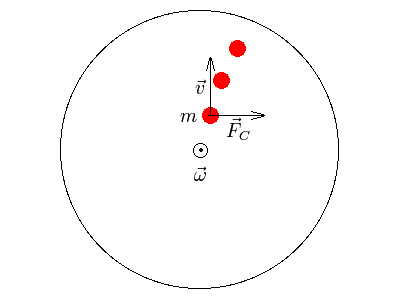
\includegraphics[height=50mm]{../images/ch04/coriolis.png}
 \caption{Siła Coriolis'a}
 \label{fig:Coriolis}
\end{figure}
Załóżmy że ciało o masie $m$ porusza się z prędkością $\vec{v}$ oraz układ w którym przemieszcza się to ciało obraca się z prędkością kątową $\vec{\omega}$. W takich warunkach ciało o którym mowa zostanie odchylone od kierunku przemieszczania się wyznaczonego przez wektor prędkości $\vec{v}$. Odchylenie to będzie spowodowane siłą Coriolis'a $\vec{F_{c}}$ którą można opisać przy pomocy wzoru \ref{eq:coriolis}. Żyroskopy MEMS wykorzystują to zjawisko określając przemieszczenie drgającego ciała, które jest tak naprawdę jedną z okładek kondensatora, jako zmianę pojemności.
\begin{equation}
  \label{eq:coriolis}
  \vec{F_{c}} = -2m \left(\vec{\omega}\times\vec{v}\right)
\end{equation}
\\
Żyroskopy tego typu posiadają dwa oscylujące miniaturowe elementy które poruszają się w przeciwnych względem siebie kierunkach (rys. \ref{fig:ZyroCoriolis}). 
\begin{figure}[!ht]
 \centering
 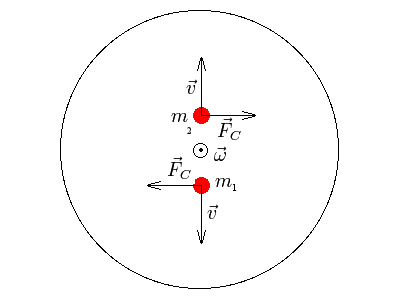
\includegraphics[height=50mm]{../images/ch04/gyro-coriolis.png}
 \caption{Dwie oscylujące masy odchylane przez siłę Coriolis'a}
 \label{fig:ZyroCoriolis}
\end{figure}
Jeżeli urządzenie do którego przymocowany jest żyroskop zacznie się obracać, spowoduje to wychylenie się oscylujących elementów w przeciwnych kierunkach. Wychylenie to z kolei powoduje zmianę pojemności, a różnica pomiędzy pojemnościami zmierzonymi przy pomocy obydwu ruchomych elementów jest proporcjonalna do prędkości kątowej. W ten sposób zmierzona szybkość obrotu jest następnie reprezentowana jako wynik analogowy (napięcie) lub cyfrowy (wartość liczbowa).
\\
Wynik działania żyroskopu MEMS jest odporny na zmianę przyspieszenia liniowego, w szczególności na przyspieszenie ziemskie. Przyspieszenie liniowe wywoła wychylenie się jednocześnie obydwu elementów oscylujących w tym samym kierunku. W ten sposób nie będzie wykryta żadna różnica pojemności. Prędkość kątowa wskazywana przez żyroskop nie ulegnie zmianie. Dzięki temu żyroskopy MEMS są odporne na wstrząsy, uderzenia oraz wibracje.
\\
Podstawowe wielkości charakteryzujące żyroskop:
\begin{itemize}
 \item zakres $[dps\footnote{dps - stopień na sekundę}]$ -- definiuje wartość maksymalną i minimalną jaką żyroskop jest w stanie
 zmierzyć. Często żyroskop ma kilka zakresów z których możemy wybrać jeden odpowiadający naszym potrzebom.
 \item czułość $[\frac{mdps}{digit}]$ -- wielkość określająca wartość minimalną jaką żyroskop może zmierzyć
 \item zmiana czułości względem temperatury $[\%]$ -- określa jak bardzo pomiary urządzenia są podatne na zmianę temperatury
 \item zakres poziomu zero $[dps]$ -- określa zakres w jakim pomiary mogą się wahać w chwili gdy żyroskop pozostaje w spoczynku
 \item zmiana zakresu poziomu zero względem temperatury $[\frac{dps}{^{\circ}C}]$ -- definiuje zmiany pomiarów żyroskopu pozostającego w spoczynku względem temperatury
 \item nieliniowość $[\% FS]$ -- parametr określa maksymalne procentowe odchylenie wartości na wyjściu żyroskopu od dopasowanej do nich linii prostej
 \item przepustowość $[Hz]$ -- definiuje częstotliwość z jaką są wykonywane pomiary
\end{itemize}

\subsubsection{Kalibracja i odczytywanie wyników}
Żyroskopy są zazwyczaj fabrycznie testowane i kalibrowane pod kątem zakresów pomiarów poziomu zerowego oraz czułości. 
Jednak umieszczeniu elementu ma płytce PCB zostaje on poddany naprężeniom przez co może być potrzebna dodatkowa kalibracja układu.

Wartości wyjściowe żyroskopu można przedstawić za pomocą równania:
\begin{equation}
  \omega_{t} = S \cdot \left(\omega_{m} - \omega_{0}\right) 
\end{equation}
\begin{tabbing}
  gdzie: \= \\
    \> $\omega_{t}$ -- rzeczywista wartość prędkości kątowa, \\
    \> $\omega_{m}$ -- pomiar z żyroskopu,\\
    \> $\omega_{0}$ -- wartość zerowa reprezentująca brak ruchu,\\
    \> $S$ -- czułość,\\
\end{tabbing}

W celu kompensacji niestabilności żyroskopu należy pozostawić urządzenie nieruchome i wykonać ok 1000 pomiarów. Następnie
konieczne jest obliczenie wartości średniej z wykonanych pomiarów. W ten sposób określimy średnie wychylenie od wartości
zerowej żyroskopu, czyli nasze $\omega_{0}$.

Podczas używania żyroskopu do pomiaru bardzo małych kątów należy jeszcze wziąć pod uwagę minimalne odchylenia wartości w
zależności od zmiany temperatury.

Prędkość kątową opisujemy wzorem: 
\begin{equation}
  \label{eq:predkosckatowa}
  \omega = \frac{d\varphi}{dt}
\end{equation}

Wzór na kąt o jaki zostało obrócone ciało poruszające się z prędkością kątową $\omega$ wyprowadzamy całkując obustronnie równanie \ref{eq:predkosckatowa}.
\begin{equation}
  \varphi = \int \omega dt
\end{equation}

Do obliczenia kąta można wykorzystać jedną z numerycznych metod całkowania, np. metodę trapezów. Metoda ta polega na podzieleniu pola pod wykresem całkowanej funkcji na wąskie trapezy, a następnie zsumowanie pól tych trapezów.

\begin{figure}[h!]
 \centering
 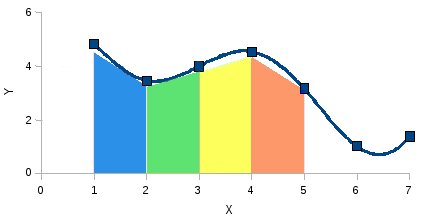
\includegraphics[height=50mm]{../images/ch04/calkowanie-metoda-trapezow.png}
 \caption{Całkowanie przy pomocy metody trapezów}
 \label{fig:CalkowanieTrapezy}
\end{figure}

Po wykorzystaniu metody trapezów, wzór na kąt o jaki żyroskop został obrócony w czasie pomiędzy dwoma pomiarami, można zapisać następująco:
\begin{equation}
  \varphi = C_{f} \cdot \frac{\omega_{i-1} + \omega_{i}}{2} \cdot \Delta t
\end{equation}
\begin{tabbing}
  gdzie: \= \\
    \> $C_{f}$ -- współczynnik korygujący, \\
    \> $\Delta t$ -- czas jaki upłynął pomiędzy dwoma pomiarami,\\
    \> $\omega_{i-1}$ -- szybkość kątowa odczytana z poprzedniego pomiaru,\\
    \> $\omega_{i}$ -- szybkość kątowa odczytana z obecnego pomiaru,\\
\end{tabbing}

W taki sposób otrzymujemy wzór na kąt całkowity pomiędzy orientacją początkowa a orientacją końcową ciała.
\begin{equation}
  \varphi_{c} = \varphi_{0} + \sum_{i=1}^{n} \varphi_{i} 
\end{equation}
\begin{tabbing}
  gdzie: \= \\
    \> $C_{f}$ -- współczynnik korygujący, \\
    \> $\Delta t$ -- czas jaki upłynął pomiędzy dwoma pomiarami,\\
    \> $\omega_{i-1}$ -- szybkość kątowa odczytana z poprzedniego pomiaru,\\
    \> $\omega_{i}$ -- szybkość kątowa odczytana z obecnego pomiaru,\\
\end{tabbing}

Do otrzymania jak najlepszych wyników konieczne jest określenie współczynnika korygującego pomiar żyroskopu.
W tym celu porównujemy wyniki pomiarów żyroskopu z pomiarami innych przyrządów np. magnetometru wykorzystując wzór:
\begin{equation}
  C_{f} = \frac{\varphi_{o}}{\varphi_{g}}
\end{equation}
\begin{tabbing}
  gdzie: \= \\
    \> $C_{f}$ -- współczynnik korygujący, \\
    \> $\varphi_{o}$ -- kąt obliczony przy pomocy urządzenia zewnętrznego,\\
    \> $\varphi_{g}$ -- kąt wyznaczony przez żyroskop,\\
\end{tabbing}

Niestety z powodu ciągle nakładających się błędów całkowania oraz niedoskonałości samego żyroskopu, wskazywany kąt odchylenia od ułożenia początkowego będzie się oddalał od wartości rzeczywistej wraz z upływem czasu. W przypadku tej pracy dyplomowej nie jest jednak potrzebna bardzo wysoka stabilność i precyzja wartości mierzonych przez żyroskop.

\subsubsection{Opis zastosowanego elementu i budowy modułu}
W robocie został użyty ultra-stabilny trójosiowy żyroskop cyfrowy L3G4200D firmy STMicroelectronics. Jego główną zaletą jest bardzo dobra jakość pomiarów osiągnięta dzięki zastosowaniu innowacyjnej struktury mechanicznej. Zazwyczaj urządzenia tego typu stosują dwie lub trzy struktury odpowiedzialne za wykonywanie pomiarów. Żyroskop firmy STMicroelectronics natomiast posiada jeden taki element odpowiedzialny za pomiar na wszystkich osiach. Takie rozwiązanie eliminuje zakłócenia pomiędzy osiami, powodowane przez same elementy pomiarowe.
\\
Zgodnie z notą katalogową\cite{L3G4200DDataSheet} żyroskop zamontowany w robocie posiada charakterystykę mechaniczną taką jak w tabeli \ref{tab:L3G4200DMechChar}:

\begin{table}[hb]
\rowcolors{2}{white}{gray!20}
\centering
\caption{Charakterystyka mechaniczna żyroskopu L3G4200D dla napięcia zasilania $3.0V$ i temperatury pracy $25^{\circ}C$}
   	\begin{tabular}{ | c | c | c | c | c | p{1.75cm} |} \hline
   		Symbol & Parametr & Warunki testowe & Wartość & Jednostka \\ \hline
   		& & & $\pm 250$ & \\
   		FS & Skala & & $\pm 500$ & dps\\
   		& & & $\pm 2000$ & \\ \hline
   		& & $FS = 250 dps$  & $8.75$  & \\
   		So  & Czułość & $FS = 500 dps$ & $17.50$  & $\frac{mdps}{digit}$ \\
   		& & $FS = 2000 dps$  & $70$  & \\ \hline
   		SoDr & Zmiana czułości & $-40^{\circ}C$ do $+85^{\circ}C$ & $\pm 2$  & \% \\
		& względem temperatury & & &  \\ \hline
		& & $FS = 250 dps$ & $\pm 10$  &  \\
   		DVoff & Zakres poziomu zero & $FS = 500 dps$  & $\pm 15$ & dps \\
   		& & $FS = 2000 dps$ & $\pm 75$ & \\ \hline
   		OffDr & Zmiana zakresu poziomu & $FS = 250 dps$  & $\pm 0.03$ & dps \\
   		& zero względem temperatury & $FS = 2000 dps$ & $\pm 0.04$ & \\ \hline
		NL & Nieliniowość & & $\pm 0.2$ & \% FS \\ \hline
		Rn & Współczynnik szumów & $BW = 50 Hz$ & $\pm 0.03$ & $\frac{dps}{\sqrt{Hz}}$ \\ \hline
		ODR & Częstotliwość odświeżania & & $100/200$ & $Hz$ \\
		& danych na wyjściu & & $400/800$ & \\ \hline
		Top & Zakres temperatur & & $-40^{\circ} C$ do $+85^{\circ} C$ & $^{\circ} C$ \\
		& operacyjnych & & & \\ \hline
   	\end{tabular}
\label{tab:L3G4200DMechChar}
\end{table}

Do żyroskopu została zaprojektowana płytka podłączeniowa PCB w programie Eagle.
\begin{figure}[!ht]
 \centering
 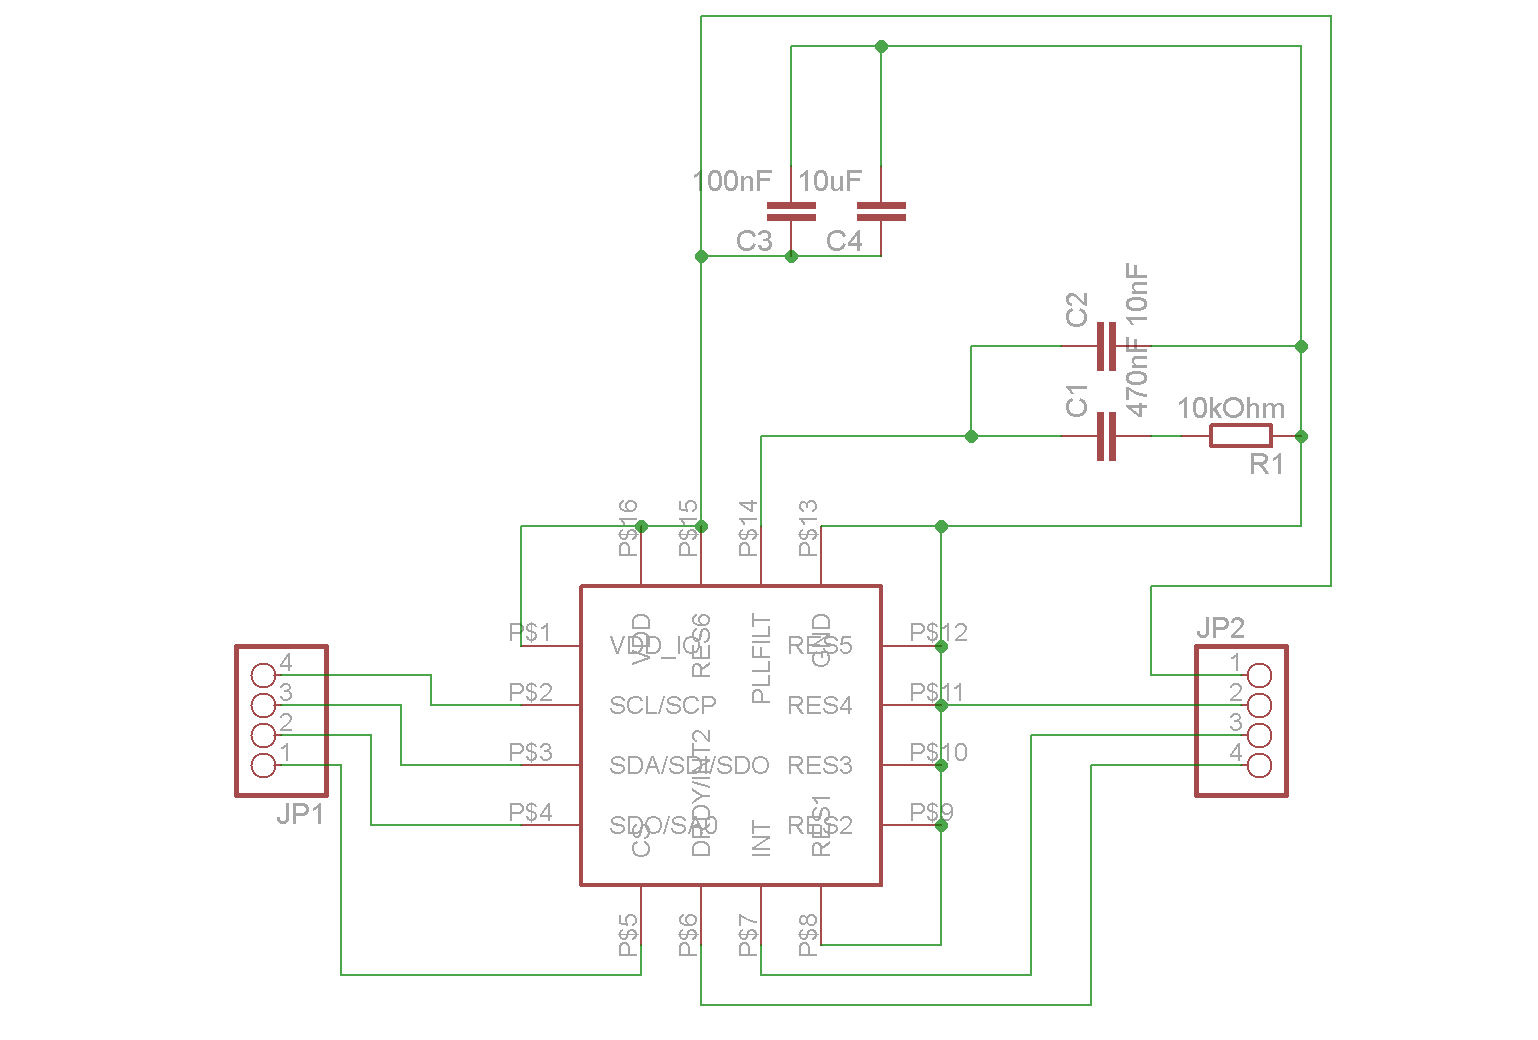
\includegraphics[height=60mm]{../images/ch04/L3G4200Dschematic.png}
 \caption{Schemat płytki PCB modułu żyroskopu}
 \label{fig:L3G4200DSchem}
\end{figure}

Schemat przedstawiony na rysunku\ref{fig:L3G4200DSchem} został stworzony na podstawie noty katalogowej.

\begin{figure}[!ht]
 \centering
 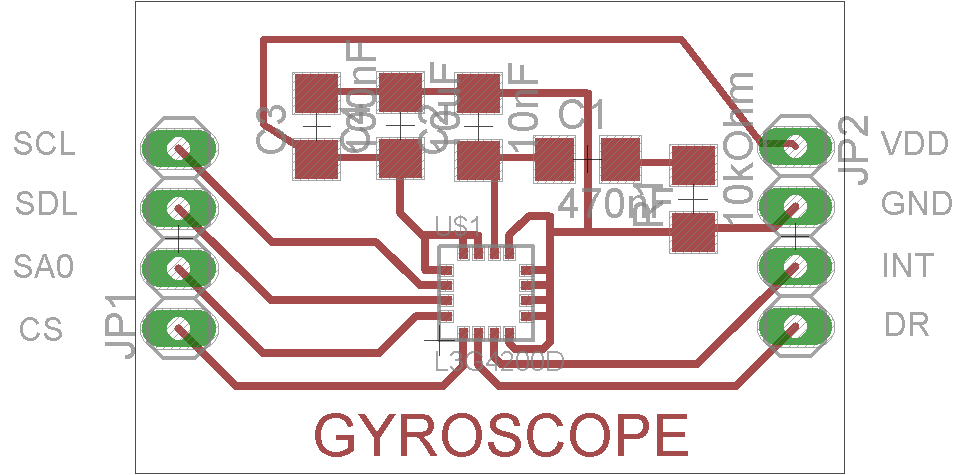
\includegraphics[height=50mm]{../images/ch04/L3G4200Dpcb.png}
 \caption{Płytka PCB modułu żyroskopu trójosiowego}
 \label{fig:L3G4200DPCB}
\end{figure}

Płytka modułu została zaprojektowana z wykorzystaniem elementów SMD w obudowie 1206. Rozmiar obudowy tych elementów został wymuszony przez brak kondensatorów ceramicznych o pojemności $10\mu F$ w obudowe mniejszej. Cały proces tworzenia płytki modułu żyroskopu był przeprowadzony metodami domowymi ze względu na koszt oraz szybkość wykonania. 
 

